\documentclass{report}
\usepackage[utf8]{inputenc}

\title{
    Titolo Progetto \\
    \large Applicazioni e Servizi Web
}

\author{Nome Autore - 000725342 \{nome.cognome@unibo.it\}}
\date{01 Gennaio 2020}

\usepackage{natbib}
\usepackage{graphicx}

\begin{document}

\maketitle
\section{Introduzione}

Il progetto proposto consiste nella realizzazione di un’applicazione web che permetta
agli utenti di creare, modificare visualizzare e condividere documenti di testo.
Il servizio permette anche di organizzare i documenti in cartelle e collaborare in tempo reale
con altri utenti sugli stessi documenti. I documenti possono essere pubblici o privati: quelli pubblici
sono visibili a tutti gli utenti della piattaforma, anche non loggati, mentre quelli privati sono visibili solo al proprietario
ed a coloro che hanno ricevuto la condivisione.

\section{Requisiti}
Prima di procedere con lo sviluppo di \textbf{Dok}, è stata effettuata un'accurata fase di analisi e definizione dei requisiti, ponendo l'utente al centro del processo di progettazione (\textit{User-Centered Design}). Dok è concepito come un sistema web-based per la gestione, la condivisione e la redazione collaborativa in tempo reale di documenti di testo, integrando funzionalità avanzate di intelligenza artificiale per l'editing di testi.

Di seguito viene riportato l'elenco dettagliato dei requisiti funzionali e non funzionali del sistema.

\subsection{Requisiti Funzionali}
I requisiti funzionali definiscono le azioni e le caratteristiche operative del sistema. Vengono suddivisi in base alle categorie di attori che interagiscono con la piattaforma.

\subsubsection{Utente Non Autenticato (Guest)}
L'utente anonimo che visita la piattaforma può:
\begin{itemize}
    \item \textbf{Registrazione:} Creare un nuovo account specificando nome, cognome, indirizzo email e password.
    \item \textbf{Autenticazione:} Effettuare l'accesso (login) al sistema per ottenere i privileges di utente registrato.
    \item \textbf{Accesso a contenuti pubblici:} Navigare nelle cartelle pubbliche e visualizzare in modalità di sola lettura i documenti contrassegnati con visibilità pubblica.
\end{itemize}

\subsubsection{Utente Autenticato}
L'utente che ha effettuato l'accesso può:
\begin{itemize}
    \item \textbf{Gestione Cartelle:} Organizzare i propri file attraverso una struttura gerarchica di cartelle nidificate. Un albero di directory che l'utente può manipolare a piacimento creando o rimuovendo nodi.
    \item \textbf{Gestione Documenti:} Gestire i documenti di testo, creandoli all'interno delle cartelle o direttamente nella radice. È prevista anche la possibilità di rinominarli ed eliminarli in modo semplice.
    \item \textbf{Visibilità Risorse:} Configurare la visibilità delle proprie risorse. Ciascuna cartella o documento nasce come privato, ma l'utente può impostarlo come pubblico in qualunque momento, rendendolo accessibile tramite un semplice URL.
    \item \textbf{Condivisione:} Collaborare condividendo i documenti con altri iscritti tramite email. Il proprietario decide se assegnare il ruolo di \textit{Viewer} (sola lettura) o \textit{Editor} (scrittura collaborativa). È fondamentale poter revocare questi permessi in qualsiasi momento.
    \item \textbf{Sistema di Notifiche:} Ricevere notifiche in tempo reale all'interno dell'interfaccia. Ad esempio quando un collega condivide un documento, o se i permessi di scrittura vengono modificati o revocati.
\end{itemize}

\subsubsection{Amministratore (Admin)}
L'utente con privilegi amministrativi può:
\begin{itemize}
    \item \textbf{Elenco Utenti:} Accedere a una dashboard centralizzata per visualizzare l'elenco completo degli utenti registrati.
    \item \textbf{Presenza Real-Time:} Monitorare in tempo reale lo stato di presenza degli utenti (se siano online o offline) e vedere l'ora dell'ultimo accesso (\textit{lastSeen}) per chi è disconnesso.
    \item \textbf{Dettagli e Metriche Utente:} Consultare le metriche di un profilo specifico, contandone i documenti creati, quelli condivisi e quelli ricevuti. Questo ci è sembrato utile per capire il livello di utilizzo delle risorse del server.
    \item \textbf{Ispezione File System:} Esaminare il file system di qualunque utente. L'amministratore può navigare tra le cartelle e i file altrui per motivi di supporto tecnico o moderazione di contenuti inappropriati.
    \item \textbf{Gestione Ruoli:} Promuovere altri utenti al ruolo di amministratore o revocare i privilegi esistenti. Il sistema avvisa in modo tempestivo l'interessato del cambio di ruolo.
\end{itemize}

\subsection{Requisiti Non Funzionali}
I requisiti non funzionali descrivono gli attributi di qualità, le prestazioni ed i vincoli a cui il sistema deve sottostare.

\begin{itemize}
    \item \textbf{Collaborazione Real-Time:} Modificare simultaneamente un documento condiviso insieme ad altri editor, con risoluzione automatica e priva di conflitti delle modifiche concorrenti.
    
    \item \textbf{Rielaborazione Testi tramite AI:} Selezionare una porzione di testo all'interno di un documento e richiedere all'assistente AI (LLM Gemini) di riscriverla in base a un'istruzione testuale fornita dall'utente.

    \item \textbf{Usabilità e Responsive Design:} L'interfaccia utente deve essere chiara, minimale e allineata ai principi KISS (\textit{Keep It Simple, Stupid}). Deve adottare una filosofia \textit{Mobile-First} per garantire una navigazione fluida ed ergonomica sia su desktop che su smartphone e tablet.
    \item \textbf{Sincronizzazione Real-Time ed Event-Based:} Lo scambio di dati in tempo reale (notifiche, aggiornamenti della dashboard e sincronizzazione dell'editing collaborativo) deve avvenire tramite un protocollo bidirezionale a bassa latenza (WebSocket), riducendo al minimo il sovraccarico di rete rispetto a tecniche di polling classico.
    \item \textbf{Risoluzione Concorrenza:} Per la stesura a più mani dei documenti si deve garantire un comportamento deterministico senza conflitti di unione (\textit{merge conflicts}), implementando strutture dati di tipo CRDT (\textit{Conflict-free Replicated Data Types}). A livello di database, la coerenza dei metadati di file e cartelle deve essere controllata tramite concurrency ottimistica.
    \item \textbf{Autenticazione e Sicurezza:} L'autenticazione deve essere gestita in modo sicuro e stateless mediante l'uso di JSON Web Token (JWT) inclusi negli header HTTP delle richieste API e trasmessi all'handshake delle WebSocket. Le password memorizzate nel database devono essere cifrate in modo irreversibile mediante algoritmo di hashing (bcrypt).
    \item \textbf{Affidabilità e Tolleranza ai Guasti:} La rilevazione della presenza degli utenti online deve gestire in modo trasparente brevi disconnessioni di rete (\textit{network flaps}) o ricaricamenti di pagina, applicando un periodo di tolleranza (\textit{grace period}) prima di dichiarare un utente disconnesso.
\end{itemize}

\section{Design}
La progettazione dell'intero sistema si focalizza sul modello iterativo basato sullo \textit{User-Centered Design}. Di seguito viene riportata l'analisi dei target user tramite la definizione di \textit{Personas} e \textit{Scenarios}, seguita dalla descrizione dell'architettura del sistema e delle interfacce utente.

\subsection{Analisi dei Target User: Personas e Scenari}
Per comprendere al meglio le esigenze dell'utenza e guidare le scelte di design e architettura, sono stati definiti tre profili utente tipo con i relativi scenari d'uso.

\begin{itemize}
    \item \textbf{Chiara (Studentessa Universitaria, 22 anni)} \\
    \textbf{Profilo:} Chiara frequenta la facoltà di Informatica e lavora spesso a progetti di gruppo. Ha bisogno di un ambiente condiviso e organizzato in cui collaborare simultaneamente con i colleghi senza rischiare conflitti di versione. \\
    \textbf{Scenario:} Chiara crea una cartella denominata "Progetto ASW" sulla piattaforma e inserisce i membri del suo gruppo. All'interno crea un documento condiviso. Durante una chiamata online, lei e i suoi colleghi aprono il documento contemporaneamente e ne redigono le varie sezioni in tempo reale, vedendo istante per istante le modifiche di ciascuno.
    
    \item \textbf{Giulia (Copywriter Freelance, 29 anni)} \\
    \textbf{Profilo:} Giulia lavora per diversi clienti scrivendo articoli e post di blog. Utilizza molto tablet e smartphone durante gli spostamenti e ha spesso bisogno di ottimizzare i tempi di scrittura, correggere bozze o ricevere spunti per rielaborare frasi complesse. \\
    \textbf{Scenario:} Giulia apre Dok dal suo tablet durante un viaggio in treno. Seleziona una porzione di testo di un articolo a cui sta lavorando e apre lo strumento di riscrittura AI integrato. Specifica un'istruzione come "Rendi il tono più formale e conciso" e invia la richiesta. Il sistema restituisce la frase riscritta, che lei inserisce direttamente nel documento.
    
    \item \textbf{Matteo (System Administrator, 35 anni)} \\
    \textbf{Profilo:} Matteo si occupa della gestione della piattaforma aziendale di documentazione basata su Dok. Ha il compito di supervisionare l'attività dei server, garantire che le risorse non vengano abusate e supportare gli utenti in caso di problemi tecnici. \\
    \textbf{Scenario:} Matteo accede alla sezione amministrativa di Dok per verificare l'affluenza sulla piattaforma. Dalla dashboard visualizza l'elenco degli utenti registrati, vedendo chi è attualmente online e chi offline. Clicca sul profilo di un utente che ha segnalato un errore e ne esamina le metriche di utilizzo e l'albero delle cartelle per identificare eventuali anomalie organizzative o problemi di permessi.
\end{itemize}

\begin{figure}[h!]
\centering
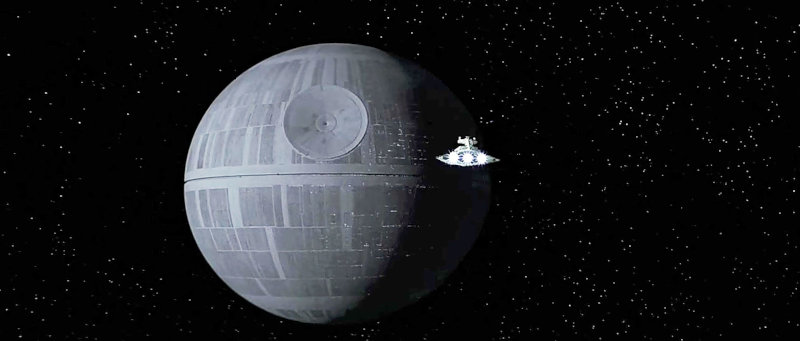
\includegraphics[scale=0.44]{deathStar2.jpg}
\caption{Death Star}
\label{fig:deathstar}
\end{figure}

\section{Tecnologie}
Tecnologie adottate e motivazioni.

\section{Codice}
Solo aspetti rilevanti.

\section{Test}
Test effettuati sul codice e test con utenti.

\section{Deployment}
Rilascio, installazione e messa in funzione.


\section{Conclusioni}
Conclusioni

\bibliographystyle{plain}
\bibliography{references}
\end{document}
